\documentclass{article}

% GRAPHICS
\usepackage{float}
\usepackage{subcaption}
\usepackage{tikz}
\usepackage{tikzscale}
\usetikzlibrary{calc}
\usepackage{graphicx}

% MATHS
\usepackage{amsmath}
\usepackage{gensymb}

\usepackage{mathtools}
\newcommand\coolover[2]{\mathrlap{\smash{\overbrace{\phantom{%
    \begin{matrix} #2 \end{matrix}}}^{\mbox{$#1$}}}}#2} 
\newcommand\coolunder[2]{\mathrlap{\smash{\underbrace{\phantom{%
    \begin{matrix} #2 \end{matrix}}}_{\mbox{$#1$}}}}#2}
    
\newcommand\coolleftbrace[2]{%
#1\left\{\vphantom{\begin{matrix} #2 \end{matrix}}\right.}

\newcommand\coolrightbrace[2]{%
\left.\vphantom{\begin{matrix} #1 \end{matrix}}\right\}#2}


% GRAPHICS
\usepackage{float}
\usepackage{subcaption}
\usepackage{tikz}
\usepackage{tikzscale}
\usetikzlibrary{calc}
\usepackage{graphicx}

% HYPERLINKS
\usepackage{hyperref}

% DOCUMENT PADDING AND MARGINS
\usepackage{titlesec}
\usepackage[margin=1.2in]{geometry}
\setlength{\parskip}{\baselineskip}%
\setlength{\parindent}{0pt}
\titlespacing*{\section}{0pt}{5ex}{2ex}
\titlespacing*{\subsection}{0pt}{1ex}{-2ex}
\titlespacing*{\subsubsection}{0pt}{2ex}{-2ex}

%COMMENTING
\usepackage{comment}


\begin{document}

% TITLE
\title{ME780 Assignment 2}
\author{Stan Brown \& Chris Choi}
\date{}
\maketitle

\section{Motion Model of a Bicycle}

\begin{figure}[H]
	\centering
	\includegraphics[width=0.6\textwidth]{images/bicycle_model.png}
	\caption{Bicycle in World Frame}
	\label{fig:bicycle}
\end{figure}

Motion of front wheel:

\begin{align}
	x_{f} &= x + L \cos(\theta) \\
	y_{f} &= y + L \sin(\theta) \\
 	\begin{bmatrix}
        x_{f, t} \\
        y_{f, t} \\
    \end{bmatrix}  
    &=
    \begin{bmatrix}
	    x_{f, t - 1} + v_{f, t} \cos(\theta_{f, t - 1} + \delta_{t}) dt \\
		y_{f, t - 1} + v_{f, t} \sin(\theta_{f, t - 1} + \delta_{t}) dt \\
    \end{bmatrix}
\end{align}

Motion of rear wheel:

\begin{align}
 	\begin{bmatrix}
        x_{r, t} \\
        y_{r, t} \\
    \end{bmatrix}  
    &=
    \begin{bmatrix}
	    x_{r, t - 1} + v_{r, t} \cos(\theta_{r, t - 1}) dt \\
		y_{r, t - 1} + v_{r, t} \sin(\theta_{r, t - 1}) dt \\
    \end{bmatrix}
\end{align}

At current we have a motion model for both the front and the rear wheel of the bicycle, however we can simplify it using the Instantaneous Center of Rotation to combine both the front and rear wheel together.

\begin{figure}[H]
	\centering
	\includegraphics[width=0.6\textwidth]{images/bicycle_icr.png}
	\caption{Simplifying the Bicycle Model with ICR}
	\label{fig:bicycle_icr}
\end{figure}

From Fig~\ref{fig:bicycle_icr} we can derive the relationship between the steering angle $\delta$ relative to the bicycle's heading:

\begin{equation}
	\label{eq:icr_steering_angle}
	\tan(\delta) = \dfrac{L}{R}
\end{equation}

Further, we know that the angular velocity $\omega$ from the point ICR of both the front and rear wheel is:

\begin{equation}
	\label{eq:icr_angluar_velocity}
	\omega = \dfrac{v \tan(\delta)}{L} = \dfrac{v}{R}
\end{equation}

Now that we have the angular velocity of the bicycle over time, the bicycle's change in heading over time is simply:

\begin{equation}
	\theta_{t} = \theta_{t - 1} + \dfrac{v_{t} \tan(\delta_{t})}{L} dt
\end{equation}

For the complete motion model of the bicycle we have:

\begin{align}
 	\begin{bmatrix}
        x_{t} \\
        y_{t} \\
        \theta_{t}
    \end{bmatrix}  
    &=
    \begin{bmatrix}
	    x_{t - 1} + v_{t} \cos(\theta_{t - 1}) dt \\
		y_{t - 1} + v_{t} \sin(\theta_{t - 1}) dt \\
		\theta_{t - 1} + \dfrac{v_{t} \tan(\delta_{t})}{L} dt
    \end{bmatrix}
\end{align}

Implementing the bicycle motion model in Matlab and simulating the motion for 20 seconds with the following parameters, we obtain a motion that resembles Fig~\ref{fig:bicycle_20s}.

\begin{itemize}	
	\vspace{-0.4cm}
	\setlength{\itemsep}{0pt}
	\setlength{\parskip}{0pt}
	\setlength{\parsep}{0pt}
	
	\item{Simulation time step $dt$: 0.1s}
	\item{Velocity $v$: $3 \text{ms}^{-1}$}
	\item{Length of bicycle $L$: 0.3m}
	\item{Steering angle $\delta$: $10 - t$ degrees}
	\item{Steering angle limit: $\pm 30$ degrees}
	\item{Standard deviation on $x$ and $y$: 0.02m}
	\item{Standard deviation on $\theta$: 1 degree}
\end{itemize}

\begin{figure}[H]
	\centering
	\includegraphics[width=0.7\textwidth]{images/bicycle_motion_20s.jpg}
	\caption{Simulating the Bicycle Model for 20s starting from (0, 0)}
	\label{fig:bicycle_20s}
\end{figure}

Just looking at Fig~\ref{fig:bicycle_20s} we can roughly validate the motion as valid, since the angle starts from +10 and ends at -10 degrees over time (20 seconds).





\newpage
\section{Carrot Controller for Bicycle}

\begin{figure}[H]
	\centering
	\includegraphics[width=0.6\textwidth]{images/carrot_controller.png}
	\caption{Carrot Controller}
	\label{fig:carrot_controller}
\end{figure}

A carrot controller is a controller that has a carrot point with a fixed distance $r$ on the trajectory line, ahead of the closest point on the trajectory line to the current robot position.


\subsection{Closest Point on the Trajectory Line to the Robot}
The closest point between the robot's position and the trajectory line can be calculated. 

\begin{figure}[H]
	\centering
	\includegraphics[width=0.5\textwidth]{images/dot_product_projection.png}
	\caption{Dot Product Projection)}
	\label{fig:dot_product_projection}
\end{figure}

Let the vector $a$ denote the vector from the start of the trajectory line to the position of the robot, and vector $b$ denote the start and end of the trajectory line. To calculate the closest point on vector $b$ to the robot position one simply has to project vector $a$ onto vector $b$, this can be calculated via:

\begin{equation}
	\text{proj}_{\vec{a}\vec{b}} 
		= \dfrac{\vec{a} \cdot \vec{b}}{|\vec{a}|}
			\dfrac{\vec{a}}{|\vec{a}|} 
		= \dfrac{\vec{a} \cdot \vec{b}}{|\vec{a}|^{2}}
			\vec{a}
\end{equation}


\newpage
\subsection{Calculation of the Carrot Point}
Once the closest point on the trajectory line to the robot is found, calculating a carrot point along the trajectory line is the closest point on the trajectory line $p_{\text{closest}}$ plus the product of look ahead distance $r$ times the unit vector of the trajectory line $b$.

\begin{equation}
	\text{carrot} = p_{\text{closest}} + r \dfrac{\vec{b}}{|\vec{b}|}
\end{equation}



\subsection{Carrot Controller}
We implemented a proportional carrot controller and traced a rectangle of $20m$ by $5m$ at $3ms^{-1}$. This is the resulting motion of the bicycle (See Fig~\ref{fig:bicycle_carrot}), we used a proportional gain $k_{p} = 2$ and look ahead distance $r$ at $2$, $0.2$ and $5$. 

From Fig~\ref{fig:bicycle_carrot} we can see that different look ahead distance $r$ impacts the way the robot traces a rectangle. If the look ahead distance is too low (i.e. Fig~\ref{fig:bicycle_carrot_bad} where $r = 0.2$), the carrot will be a very small distance ahead of the robot, making small adjustments unlikely thereby the angle of the steering oscillates between $-30$ degrees to $30$ degrees (the max steering angle).

If the carrot is at a medium look ahead distance away from the robot  (i.e. Fig~\ref{fig:bicycle_carrot_ok} where $r = 2$), the robot tends to be quite agreessive in compensating for overshooting the trajectory. As we increase the look ahead distance $r$ however, the correction angle is dampened, causing a less agreessive correction, but longer time to return to the trajectory line.

\begin{figure}[H]
	\centering
	
	\begin{subfigure}[b]{\linewidth}
		\centering
		\includegraphics[width=0.5\textwidth]{images/bicycle_carrot_bad.jpg}
		\caption{$k_{p} = 2$, $r = 0.2$}
		\label{fig:bicycle_carrot_bad}
	\end{subfigure}
		
	\begin{subfigure}[b]{\linewidth}
		\centering
		\includegraphics[width=0.5\textwidth]{images/bicycle_carrot.jpg}
		\caption{$k_{p} = 2$ and $r = 2$}
		\label{fig:bicycle_carrot_ok}
	\end{subfigure}
	
	\begin{subfigure}[b]{\linewidth}
		\centering
		\includegraphics[width=0.5\textwidth]{images/bicycle_carrot_better.jpg}
		\caption{$k_{p} = 2$, $r = 5$}
		\label{fig:bicycle_carrot_better}
	\end{subfigure}
	
	\caption{Bicycle motion using carrot controller starting at (23, 10)}
	\label{fig:bicycle_carrot}
\end{figure}



\newpage
\section{IGVC Planner}
\label{sec:igvc_planner}
We were given a map of the Intelligent Ground Vehicle Competition in the form of a $926 \times 716$ element grid, where each cell
represents a 10 cm X 10 cm area of the course, creating a 92.6 m X 71.6 m environment. 

Our goal is to implement a planner and present a combined motion planning solution that finds a straight-line path through the environment, then uses the carrot planner to locally drive the vehicle to the goal location. Where the start and end locations are ($4.0m$, $0.5m$, $3.14159 rad$) and ($5.0 m$, $1.0 m$, not defined) for $x$, $y$ and $θ$.


\begin{figure}[H]
	\centering
	\includegraphics[width=0.7\textwidth]{images/IGVCmap.jpg}
	\caption{IGVC Map}
	\label{fig:igvc_map}
\end{figure}



\newpage
\subsection{Wavefront Planner}
\label{subsec:wavefront}
Since the map given represents an occupancy grid of free space and obstacles, our intial approach was to use the breadth first search based planner, by using the wavefront method to calculate the cost distance to traverse from start to goal point, and finding the lowest cost path. In Fig~\ref{fig:wavefront} you can see the result of one wavefront plan and the lowest cost path leading from the start to goal point.

\begin{figure}[H]
	\centering
	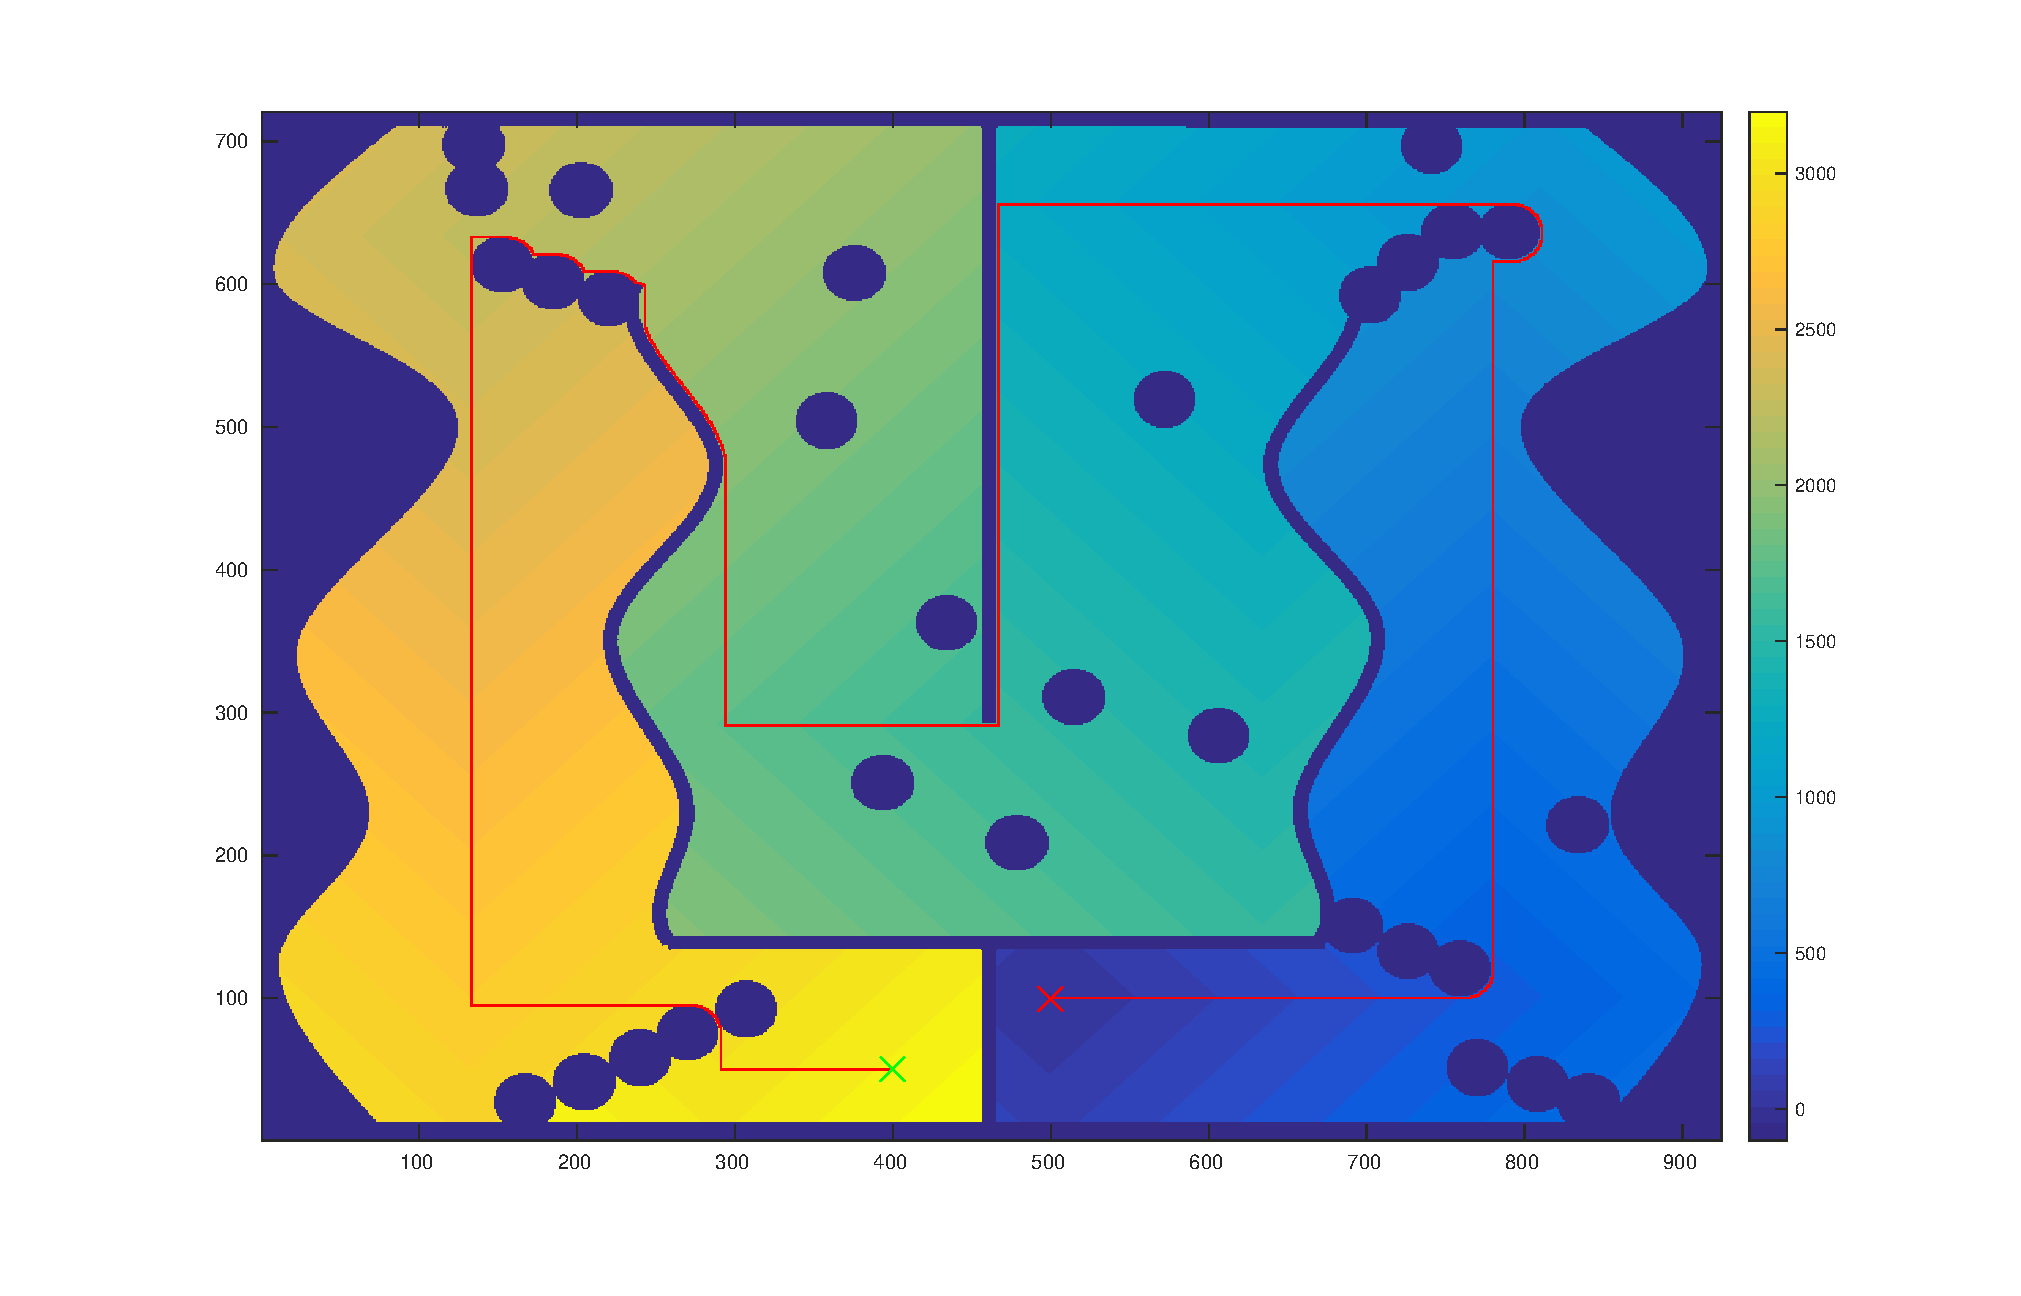
\includegraphics[width=0.9\textwidth]{images/wavefront_igvc.eps}
	\caption{Wavefront IGVC Map}
	\label{fig:wavefront}
\end{figure}

The problem with wavefront is as follows:

\begin{itemize}
	\item{\textbf{Manhattan Distance}: Due to the nature of how the wavefront traverses the map, the paths found have inherently right angle turns, using a carrot controller following paths with right angles can be problematic.}
	
	\item{\textbf{Difficult to represent robot}: This is not limited to the wavefront method, but for any occupancy grid planner methods, the grid size should be smaller than the robot.}
	
	\item{\textbf{Exploits holes in map}: Holes between objects can be a problem such as Fig~\ref{fig:wavefront}, near the start point wavefront finds a small gap between the circular obstacles, however, in reality the physical robot will not be able to fit through the gap.}
\end{itemize}

In conclusion, we gave up on the wavefront planner because the paths produced were not suitable for the carrot controller.



\newpage
\subsection{Probablistic Roadmap Planner}
\label{subsec:prm}
In our next approach we used the Probablistic Roadmap (PRM) planner, purely out of curiosity and it seemed like an intuitive alternative to wavefront planner. 

For the implementation we had to make modifications to the PRM example code given, as the code given assumes the obstacles are in the form of polygon points, the example code makes use of Matlab's `inpolygon()` function to detect whether a sample point is within a polygon. However the map given represents an occupancy grid instead of the obstacle polygons as points, we therefore had to replace the collision checking to use a ray tracing algorithm such as Bresenham's line algorthm, so that we can traverse between the PRM sample points and create collision free edges.

\begin{figure}[H]
	\centering
	\begin{subfigure}[b]{0.49\linewidth}
		\centering
		\includegraphics[width=\textwidth]{images/prm_200.jpg}
		\caption{200 Samples}
	\end{subfigure}
	\begin{subfigure}[b]{0.49\linewidth}
		\centering
		\includegraphics[width=\textwidth]{images/prm_500.jpg}
		\caption{500 Samples}
	\end{subfigure}
	
	\begin{subfigure}[b]{0.49\linewidth}
		\centering
		\includegraphics[width=\textwidth]{images/prm_1000.jpg}
		\caption{1000 Samples}
	\end{subfigure}
	\begin{subfigure}[b]{0.49\linewidth}
		\centering
		\includegraphics[width=\textwidth]{images/prm_5000.jpg}
		\caption{5000 Samples}
	\end{subfigure}
	\caption{PRM Planner and Carrot Controller}
	\label{fig:prm}
\end{figure}

\newpage
From Fig~\ref{fig:prm} we show the combination of PRM and carrot controller through the IGVC map with varying number of samples (200, 500, 1000, 5000). While 200 sample points was sufficient, it is easy to recognize the path as sub-optimal compared to the paths generated with 500 sample points and beyond, we can observe that the path gets more and more optimal as we increase the number of sample points in the map.


\subsubsection{PRM Planner with Sample Points Padded}
\label{subsec:prm_padding}
We attempted to make improvements with the PRM approach so that the bicycle forward motion does not collide with the obstacles, we improved the PRM planner by ensuring the sample points are a set distance away from the obstacles, this is done by performing a line search on 8 directions (N, NE, E, SE, S, SW, W, NW), if collision is detected the sample point is dropped.

\begin{figure}[H]
	\centering
	\includegraphics[width=\linewidth]{images/prm_resampling.jpg}
	\caption{PRM Resampling}
	\label{fig:prm_resampling}
\end{figure}


\section{Limitations and Future Improvements to the PRM Planner}
\subsection{Limitations}
Previously in Section~\ref{sec:igvc_planner} we have explored both wavefront and PRM path planning methods, both methods alone are not satifactory in planning a path for the bicycle through the IGVC course, we will discuss three limitations below:


\begin{itemize}
	\item{\textbf{Path is not smooth}: The paths generated by both wavefront and PRM while optimal it does not take into account the motion model of the bicycle. Some of the planned paths particularly nearer towards the middle of the course where the bicycle has to make a U-turn, the angle change is very sharp and sudden, improvement in either the controller or path planned should take the motion model into account and create a smooth path or motion through the turn.}
	
	\item{\textbf{No collision detection}: The above two methods does not perform collision dection of the robot with regards to the obstacles in the map, there are methods such as trajectory rollout that iterates at every timestep performing collision check at every possible motion change to make sure the path is valid.}
	
	\item{\textbf{Wasted Computation Around Non-Optimal Areas}:}
	
\end{itemize}

\begin{figure}[H]
	\centering
	\includegraphics[width=\linewidth]{images/collision_example.jpg}
	\caption{Collision Example}
	\label{fig:collision_example}
\end{figure}


\subsection{Future Improvements}
While padding was useful, it suffers around the choke points in the map (figure example...).

Trajectory roll out please...




\end{document}